\section{Design}
FlashEigen is an external-memory eigensolver framework optimized for any fast
I/O devices
such as a large SSD array to compute eigenvalues of sparse graphs (Figure
\ref{arch}). We build FlashEigen on top of SAFS, a user-space filesystem,
to fully utilize the I/O throughput of a large SSD array. Instead of
implementing eigenvalue algorithms from scratch, we integrate FlashEigen
with the Anasazi framework to compute eigenvalues. The Anasazi framework
implements multiple state-of-art eigenvalue algorithms and provides users
a flexible programming interface to redefine both sparse and dense matrix
operations required by the eigenvalue algorithms. FlashEigen stores both sparse
and dense matrices in SAFS and focuses on optimizing the matrix operations
required by the Anasazi eigensolvers for SSDs.

\begin{figure}
\centering
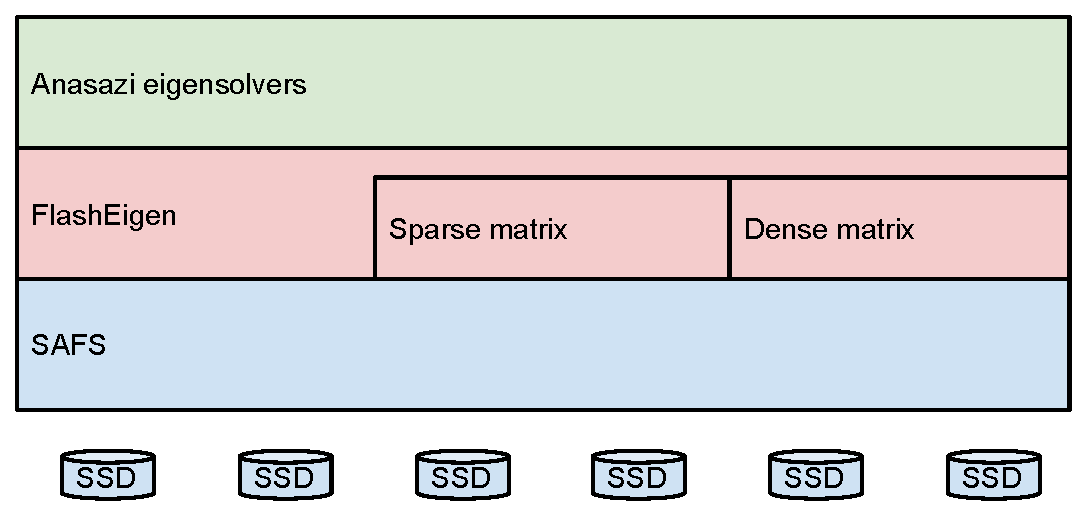
\includegraphics[scale=0.4]{./architecture.pdf}
\vspace{-5pt}
\caption{The architecture of FlashEigen.}
\vspace{-5pt}
\label{arch}
\end{figure}

\subsection{Eigensolver algorithm}

%\begin{figure}
%\centering
%\includegraphics[scale=0.35]{./SpMM.pdf}
%\vspace{-5pt}
%\caption{}
%\vspace{-5pt}
%\label{SpMM}
%\end{figure}

\begin{algorithm}
	\begin{algorithmic}[1]
		\For{i = 0, 1, ..., until convergence}
		\State (1) Update the subspace $S \in \mathbb{R}^{n \times m}$,
		\State (2) Solve the projected eigenproblem $S^TASy = S^TSy\theta$.
		\State (3) Compute the residual: $r = Kx - x\theta$, where
		\State\hspace{\algorithmicindent} $x = Sy$ (Ritz vector), $\theta = \rho(x)$ (Ritz value).
		\State (4) Test the convergence of a Ritz pair $(x, \rho(x))$.
		\EndFor
	\end{algorithmic}
	\caption{Pseudo code of a generic eigenvalue algorithm that compute eigenvalues
	of a square matrix $A$ with $n$ rows and columns.}
	\label{eigencode}
\end{algorithm}

The state-of-art eigenvalue algorithms compute eigenvalues with iterative
methods. Algorithm \ref{eigencode} shows the general steps used by the eigenvalue
algorithms.
Step (1) constructs a vector subspace $S \in \mathbb{R}^{n \times m}$, where
$n$ is the number of rows and columns of a sparse matrix and $m$ is the number
of vectors in the subspace. When computing eigenvalues of a sparse graph,
two key operations in this step are sparse matrix multiplication to construct
the subspace and reorthogonalization to correct floating-point rounding errors.
Step (2) projects the large sparse matrix to a much smaller matrix with only
$m$ rows and $m$ columns, which can be solved by other eigensolvers such as
the one in LAPACK \cite{lapack}. Step (3) projects the solution of the small
eigenvalue problem back to the original eigenvalue problem. Step (4) tests
whether the projected solution fulfills the precision requirement given by
users. If not, the algorithm adjusts the vector subspace, returns to step (1)
and continues the process.

The block extenion implemented in the Anasazi eigensolvers updates multiple
vectors in the subspace in an iteration. This optimization leads to sparse
matrix dense matrix multiplication, which increases computation density to
improve performance, as well as a set of dense matrix operations instead of
vector operations. The number of vectors to be updated together is determined
by the \textit{block size}, denoted by $b$. The subspace size $m$
is $b \times NB$, where $NB$ is the number of blocks.

\subsection{SAFS}

SAFS \cite{safs} is a user-space filesystem for a high-speed SSD array in
a NUMA (non-uniform memory architecture) machine. It is implemented as
a library and runs in the address space
of its application. It is deployed on top of the Linux native filesystem.
SAFS was originally designed for optimizing small I/O accesses. However,
sparse matrix multiplication and dense matrix operations
generate much fewer but much larger I/O. Therefore, we provide additional
optimizations to maximize sequential I/O throughput from a large SSD array.

The original SAFS has a dedicated I/O thread for each SSD. The I/O thread
accesses the SSD exclusively to avoid lock contention in the Linux kernel.
Application threads have to send I/O requests to one of the I/O threads
with message passing when accessing data from SSDs. It is necessary to have
one I/O thread for
an SSD when applications issue many small I/O accesses because processing
a large number of I/O accesses consumes a significant number of CPU cycles.
However, when the workload only has large I/O requests, each I/O request takes
much longer time to complete. As a result, the I/O threads are constantly put
into sleep while waiting for I/O and each I/O completion may suffer from
the latency of a thread context switch.

The latency of a thread context switch becomes noticeable on a high-speed SSD
array under a sequential I/O workload and it becomes critical to avoid thread
context switch to gain I/O performance. Therefore, instead of having an I/O
thread for each SSD, we use only a single I/O thread for each NUMA node, which
is responsible for all of the SSDs connected to the NUMA node. As such, an I/O
thread processes many more I/O requests to amortize the latency of a context
switch. Similarly, application threads communicate with I/O threads through
message passing when issuing I/O requests. If the computation in application
threads did not saturate CPU, SAFS would put the application threads into
sleep while they were waiting for I/O. This results in many thread context
switches and underutilization of both CPU and SSDs. To saturate I/O,
an application thread issues asynchronous I/O and poll for I/O to avoid thread
context switches after completing all computation available to it.

To better support access to many relatively small files simultaneously, SAFS
stripes data in a file across SSDs with a different striping order for each file.
This strategy stores data from multiple files evenly across SSDs and improves
I/O utialization. Due to the sequential I/O workload, FlashEigen stripes data
across SSDs with a large block size, on the order of megabytes, to increase I/O
throughput and potentially reduce write amplification on SSDs \cite{Tang15}.
Such a large block size may cause storage skew for small files
on a large SSD array if every file stripes data in the same order. Using
the same striping order for all files may also cause skew in I/O access.
Therefore, SAFS generates a random striping order for each file to evenly
distribute I/O among SSDs when a file is created. SAFS stores the striping
order with the file for future data retrieval.

\subsection{Sparse matrix multiplication} \label{spmm}
Sparse matrix multiplication is one of the most computationally expensive
operations in an eigensolver. Applying this operation on real-world graphs
usually leads to many random memory accesses and its performance is usually
limited by the random memory performance of DRAM. The block extension
in the Anasazi eigensolvers enables sparse matrix dense matrix multiplication
to increase data locality and computation density and improve overall performance
of an eigensolver.

To scale sparse matrix multiplication to a sparse graph with billions of vertices,
we perform this operation in semi-external memory (SEM). That is, we keep dense
matrices in memory and the sparse
matrix on SSDs. This strategy enables nearly in-memory performance while achieving
the scalability in proportion to the ratio of edges to vertices in a graph.

\subsubsection{The sparse matrix format}
The state-of-art numeric libraries store a sparse matrix in compressed row storage
(CSR) or compressed column storage (CSC) format. However, these formats incur
many CPU cache misses in sparse matrix multiplication on many real-world graphs
due to their nearly random vertex connection. They also require a relatively
large storage size. For a graph with billions of edges, we have to use eight
bytes to store the row and column indices. For semi-external memory sparse
matrix multiplication, SSDs may become the bottleneck if a sparse matrix has
a large storage size.
Therefore, we need to use an alternative format for sparse matrices to increase
CPU cache hits and reduce the amount of data read from SSDs.

\begin{figure}
\centering
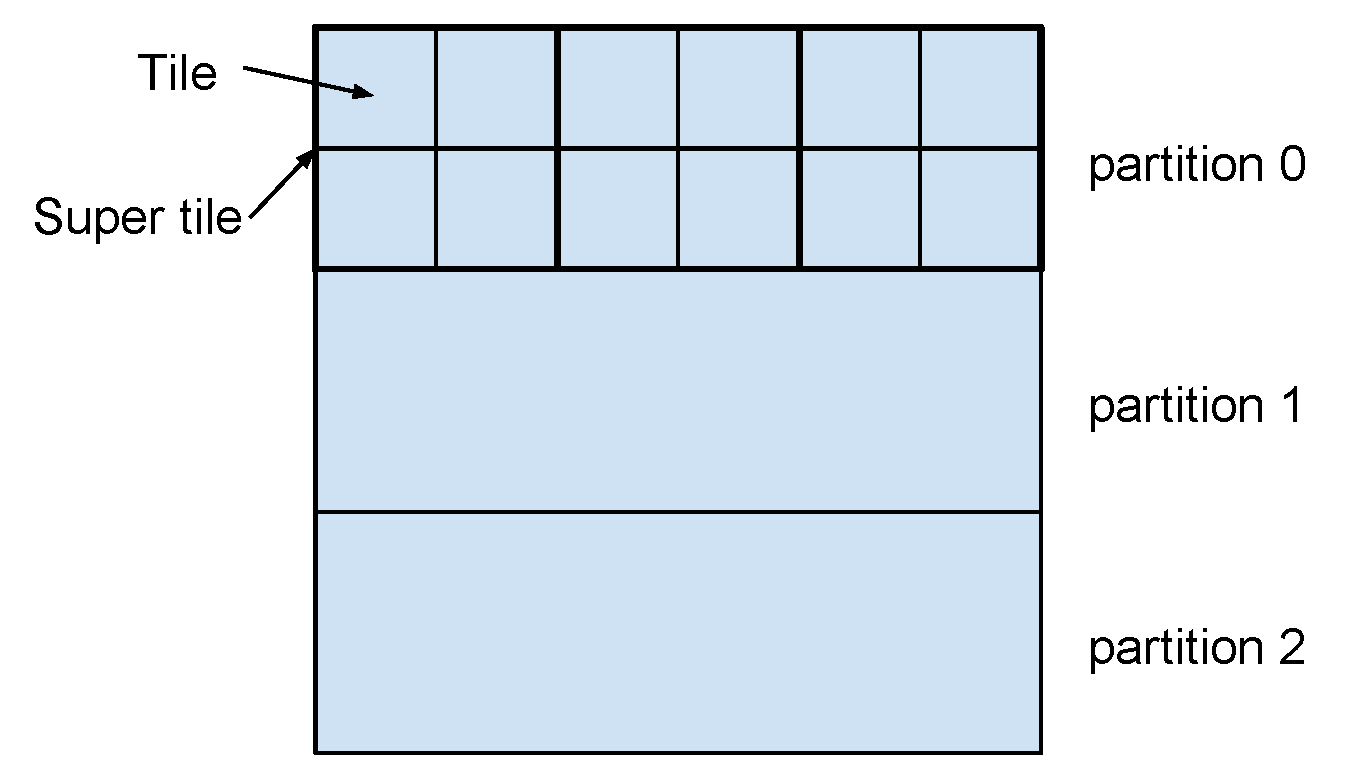
\includegraphics[scale=0.3]{./sparse_mat.pdf}
\vspace{-5pt}
\caption{The format of a sparse matrix in FlashEigen.}
\vspace{-5pt}
\label{sparse_mat}
\end{figure}

To increase CPU cache hits, we deploy cache blocking \cite{Im04} and store
non-zero entries of a sparse matrix in tiles (Figure \ref{sparse_mat}).
When a tile is small, the rows from the input and output dense matrices
involved in the multiplication with the tile are always kept in the CPU cache
during the multiplication. The optimal tile size should fill the CPU cache
with the rows of the dense matrices involved in the multiplication with
the tile and is affected by the number of columns of the dense matrices,
which is chosen by users. Instead of generating a sparse matrix with
different tile sizes optimized for different numbers of columns in the dense
matrices, we use a relatively small tile size and rely on the runtime system
to optimize for different numbers of columns (in section \ref{sec:exec}).
In the semi-external memory, we expect that the dense matrices do not
have more than eight columns in sparse matrix multiplication. Therefore, we
use the tile size of $16K \times 16K$ by default to balance the matrix storage
size and the adaptibility to different numbers of columns.

\begin{figure}
\centering
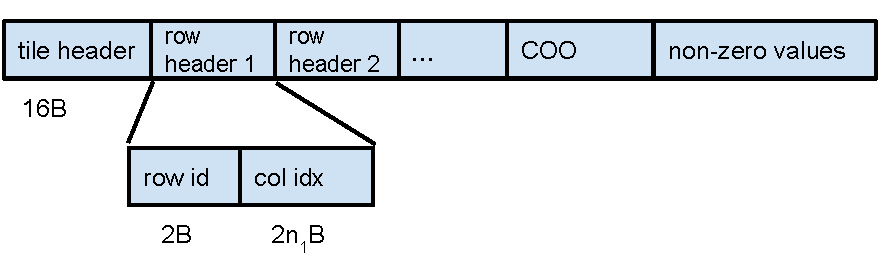
\includegraphics[scale=0.5]{./tile_format.pdf}
\vspace{-5pt}
\caption{The storage format of a tile in a sparse matrix.}
\vspace{-5pt}
\label{tile_format}
\end{figure}

To reduce the overall storage size of a sparse matrix, we use a compact format
to store non-zero entries in a tile. In very sparse matrices such as
many real-world graphs, many rows in a tile do not have any non-zero entries.
The CSR (CSC) format requires an entry for each row (column) in the row
(column) index. Therefore, the CSR or CSC format wastes space when storing elements
in a tile. Instead, we only keep data for rows with non-zero entries in a tile
shown in Figure \ref{tile_format} and refer to this format as SCSR (Super
Compressed Row Storage). This format maintains a row header for each non-empty
row. A row header has an identifier to indicate the row number, followed by
column indices. 
The most significant bit of the identifier is always set to 1, while the most
significant bit of a column index entry is always set to 0. As such, we can easily
distinguish a row identifier from a column index entry and determine the end
of a row. Thanks to the small size of a tile, we use two bytes to further store a row
number and a column index entry to reduce the storage size. Since the most
significant bit is used to indicate the beginning of a row, this format allows
a maximum tile size of $32K \times 32K$.

For many real-world graphs, many rows in a tile have only one non-zero entry,
thanks to the sparsity of the graphs and nearly random vertex connection.
Iterating over single-entry rows requires to test the end of a row for every
non-zero entry, resulting in many extra conditional jump CPU instructions
in sparse matrix multiplication.
In contrast, the coordinate format (COO) is more suitable for storing these
single-entry rows. It does not increase the storage size but significantly
reduces the number of conditional jump instructions when we iterate
them. As a result, we hybrid SCSR and COO to store non-zero entries in a tile
with COO stored behind the row headers of SCSR. All non-zero entries are
stored together at the end of a tile.

We organize tiles in a sparse matrix in tile rows and maintain a matrix index
for them. Each entry of the index stores the location of a tile row on SSDs
to facilitate random access
to tile rows. This is useful for parallelizing sparse matrix multiplication.
Because a tile contains thousands of rows, the matrix index requires a very
small storage size even for a billion-node graph. We keep the entire index
in memory during sparse matrix multiplication.

\subsubsection{The dense matrix format for SpMM} \label{numa_mat}
Dense matrices in sparse matrix multiplication are tall-and-skinny (TAS)
matrices
with millions or even billions of rows but only several columns. The number
of rows in a dense matrix is determined by the number of vertices in a sparse
graph and the number of columns is determined by the \textit{block size}
in an eigensolver with the block extension. The dense matrix is kept in memory
for semi-external memory (SEM) sparse matrix dense matrix multiplication (SpMM),
so the size of the dense matrix governs the memory consumption
of SpMM. Given the limited amount of RAM in a machine, the number of columns
in a dense matrix has to be small.

For a non-uniform memory architecture (NUMA), we partition the input dense matrix
horizontally and store partitions evenly across NUMA nodes to fully utilize
the bandwidth of memory and inter-processor links in sparse matrix
multiplication. The NUMA architecture is prevalent in today's multi-processor
servers, where each processor connects to its own memory banks. As shown in
Figure \ref{dense_mat} (a), we assign multiple
contiguous rows in a row interval to a partition, which is assigned to a NUMA
node. A row interval always has $2^i$ rows for efficiently locating a row
with bit operations. The row interval size is also multiple of the tile size of
a sparse matrix so that multiplication on a tile only needs to access rows
from a single row interval. We store elements in a row interval in row-major
order to increase data locality in SpMM.

\begin{figure}
\centering
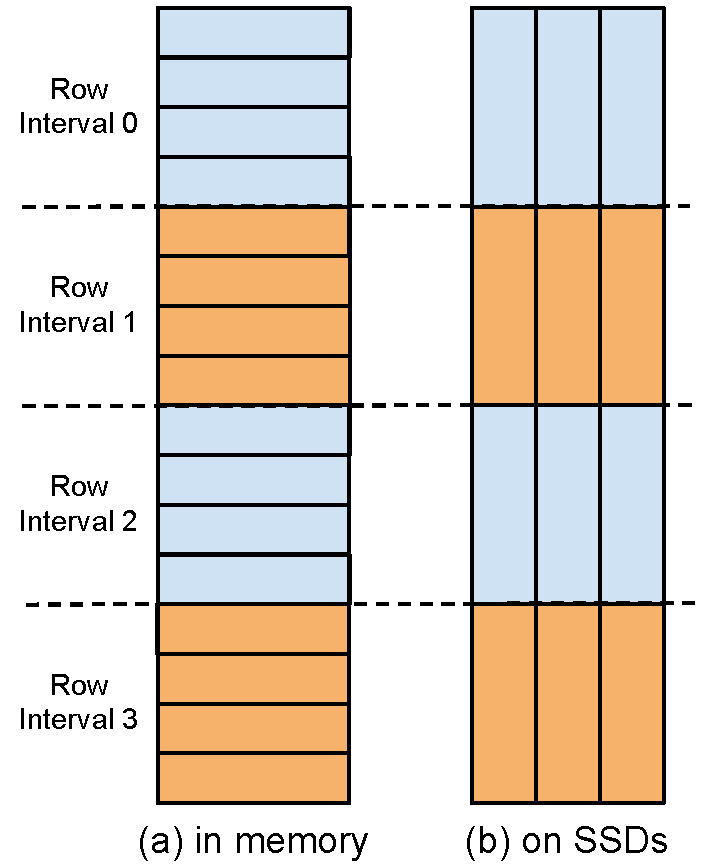
\includegraphics[scale=0.4]{./dense_matrix.pdf}
\vspace{-5pt}
\caption{The data layout of tall-and-skinny (TAS) dense matrices. A TAS
dense matrix is partitioned horizontally into many row intervals.
(a) For an in-memory matrix, row intervals are stored across NUMA nodes and
elements are stored in row-major order; (b) for an SSD-based matrix, elements
inside a row interval are stored in column-major order.}
\vspace{-5pt}
\label{dense_mat}
\end{figure}

\subsubsection{Execution of sparse matrix multiplication} \label{sec:exec}
We perform sparse matrix dense matrix multiplication in semi-external memory
and optimize it for different numbers of columns in the dense matrices.
Thanks to the semi-external memory execution, sparse matrix multiplication
streams data in the sparse matrix from SSDs, which maximizes I/O throughput
of the SSDs.

We partition a sparse matrix horizontally for parallelization and assign multiple
contiguous tile rows to the same partition (Figure \ref{sparse_mat}).
The number of tile rows assigned to a partition is determined at runtime
based on the number of columns in the input dense matrix. A thread reads
a partition of the sparse matrix asynchronously from SSDs. Once a partition
is ready in memory, the worker thread multiplies the partition with the input
dense matrix. A thread processes one tile at a time and stores
the intermediate result in a buffer allocated in the local memory to reduce
remote memory access. %To reduce memory consumption,
%we write the portion of the output dense matrix to SSDs immediately whenever
%it is generated. \dz{Implement this.}

To better utilize CPU cache, we process tiles of a partition in
\textit{super tile}s (Figure \ref{sparse_mat}). The tile size of a sparse
matrix is specified when the sparse matrix image is created and is relatively
small to handle different numbers of columns in the dense matrices.
A \textit{super tile} is composed of tiles from multiple tile rows and its
size is determined at runtime by three factors: the number of columns
in the dense matrices, the CPU cache size and the number of threads that
share the CPU cache. An optimal size for a \textit{super tile} fills
the CPU cache with the rows from the dense matrices involved in
the computation with the \textit{super tile}.

Load balancing also plays a key role in sparse matrix multiplication on
many real-world graphs due to their power-law distribution in vertex degree.
In FlashEigen, a worker thread first processes partitions originally assigned
to the thread. When a worker thread finishes
all of its own partitions, it steals partitions that have not been processed
from other worker threads.

In spite of nearly random edge connection in a real-world graph,
there exists regularity that allows vectorization to improve performance
in sparse matrix dense matrix multiplication. For each non-zero entry, we
need to multiply it with the corresponding row from the input dense matrix
and add the result to the corresponding row in the output dense matrix.
These operations can be accomplished by the vector CPU instructions such as
AVX \cite{avx}. The current implementation relies on GCC's auto-vectorization
to translate the C code to the vector CPU instructions by predefining the matrix
width in the code.

When accessing a sparse matrix on SSDs, we keep a set of memory buffers for
I/O access to reduce the overhead of memory allocation.
For a large spare matrix, each tile row is fairly large, on the order
of tens of megabytes. The operating system usually allocate a memory buffer
for such an I/O size with \textit{mmap()} and populates the buffer with physical
pages when the buffer is used. It is computationally expensive to populate
large memory buffers frequently. When accessing high-throughput I/O devices,
such overhead can cause substantial performance loss. Therefore, we keep a set
of memory buffers allocated previously and reuse them for new I/O requests.
Because tile rows in a sparse matrix usually have differnt sizes, we resize
a previously allocated memory buffer if it is too small for a new I/O request.

\subsection{The vector subspace}
The vector subspace required by an eigensolver is massive when the eigensolver
computes eigenvalues of a billion-node graph or computes many eigenvalues
of a multi-million-node graph. The number of vectors in the subspace
increases with the number of required eigenvalues. Furthermore, a larger
number of vectors in the subspace potentially improves the convergence rate
of an eigensolver. The storage size required by the subspace is often larger than
the sparse matrix for eigendecomposition on many real-world graphs. Therefore,
FlashEigen stores these vectors on SSDs.

\begin{table}
	\begin{center}
		\small
		\begin{tabular}{|c|c|c|c|c|}
			\hline
			name & operation & customized output \\
			\hline
			\textit{MvTimesMatAddMv} & $CC \leftarrow \alpha \times AA \times B + \beta \times CC$ & yes \\
			\hline
			\textit{MvTransMv} & $A \leftarrow \alpha \times t(AA) \times BB$ & no \\
			\hline
			\textit{MvScale1} & $BB \leftarrow \alpha \times AA$ & yes \\
			\hline
			\textit{MvScale2} & $BB \leftarrow AA \times diag(vec)$ & yes \\
			\hline
			\textit{MvAddMv} & $CC \leftarrow \alpha \times AA + \beta \times BB$ & yes \\
			\hline
			\textit{MvDot} & $vec[i] \leftarrow t(AA[,i]) * BB[,i]$ & no \\
			\hline
			\textit{MvNorm} & $vec \leftarrow norm\_col(AA)$ & no \\
			\hline
			\textit{CloneView} & $AA[,idxs]$ & yes \\
			\hline
			\textit{SetBlock} & $AA[,idxs] \leftarrow BB$ & yes \\
			\hline
			\textit{MvRandom} & $AA \leftarrow rand\_init$ & yes \\
			\hline
			\textit{ConvLayout} & $AA \leftarrow conv\_layout(BB)$ & yes \\
			\hline
		\end{tabular}
		\normalsize
	\end{center}
	\caption{The dense matrix operations required by the Anasazi eigensolvers.
		$AA$ and $BB$ represents a tall dense matrix, $A$ and $B$ represents
		a small dense matrix, $\alpha$ and $\beta$ represents scalar variables.}
	\label{anasazi_ops}
\end{table}

FlashEigen implements a set of dense matrix operations shown in Table
\ref{anasazi_ops}. The Anasazi framework provides a set of programming
interfaces that expose the vectors in the subspace to users as dense matrices
and allow users to redefine the dense matrices and the operations on them.
The first ten operations are the ones required by the Anasazi
framework. The most computationally expensive operations are the two
matrix multiplication operations: \textit{MvTimesMatAddMv} and \textit{MvTransMv},
mainly used for reorthogonalization to fix floating-point rounding errors.
The eigensolvers use \textit{CloneView} and \textit{SetBlock} to access individual
columns of a dense matrix, so we store the dense matrices in column major by default.
However, the sparse matrix dense matrix multiplication described in Section
\ref{spmm} requires a row-major dense matrix to increase data locality. Thus,
FlashEigen adds another operation \textit{ConvLayout} to convert data layout
in dense matrices, which converts a column-major matrix to a row-major
matrix when it is passed to the SpMM operation.

External-memory dense matrix operations faces multiple challenges.
Unlike sparse matrix multiplication, these dense matrix operations are less
memory intensive. Even though SSDs are fast, their sequential I/O performance
is still an order of magnitude slower than RAM. Furthermore, SSDs wears out
after a certain amount of write. Even enterprise SSDs \cite{ocz} only allows
a small number of DWPD
(diskful writes per day). Therefore, FlashEigen optimizes dense matrix operations
with three goals: \textit{(i)} maximizing I/O throughput of SSDs, \textit{(ii)}
minimizing the amount of data read from SSDs, \textit{(iii)} reducing SSD
wearout.

%\begin{figure}
%	\begin{center}
%		\footnotesize
%		\vspace{-15pt}
%		\begin{tikzpicture}[gnuplot]
%% generated with GNUPLOT 4.6p4 (Lua 5.1; terminal rev. 99, script rev. 100)
%% Thu 16 Jul 2015 09:41:54 AM EDT
\path (0.000,0.000) rectangle (8.382,4.572);
\gpcolor{color=gp lt color border}
\gpsetlinetype{gp lt border}
\gpsetlinewidth{1.00}
\draw[gp path] (1.320,0.616)--(1.500,0.616);
\draw[gp path] (7.829,0.616)--(7.649,0.616);
\node[gp node right] at (1.136,0.616) { 0};
\draw[gp path] (1.320,1.436)--(1.500,1.436);
\draw[gp path] (7.829,1.436)--(7.649,1.436);
\node[gp node right] at (1.136,1.436) { 5};
\draw[gp path] (1.320,2.256)--(1.500,2.256);
\draw[gp path] (7.829,2.256)--(7.649,2.256);
\node[gp node right] at (1.136,2.256) { 10};
\draw[gp path] (1.320,3.075)--(1.500,3.075);
\draw[gp path] (7.829,3.075)--(7.649,3.075);
\node[gp node right] at (1.136,3.075) { 15};
\draw[gp path] (1.320,3.895)--(1.500,3.895);
\draw[gp path] (7.829,3.895)--(7.649,3.895);
\node[gp node right] at (1.136,3.895) { 20};
\draw[gp path] (2.250,0.616)--(2.250,0.796);
\draw[gp path] (2.250,3.895)--(2.250,3.715);
\node[gp node center] at (2.250,0.308) {op1};
\draw[gp path] (3.180,0.616)--(3.180,0.796);
\draw[gp path] (3.180,3.895)--(3.180,3.715);
\node[gp node center] at (3.180,0.308) {op2};
\draw[gp path] (4.110,0.616)--(4.110,0.796);
\draw[gp path] (4.110,3.895)--(4.110,3.715);
\node[gp node center] at (4.110,0.308) {op3};
\draw[gp path] (5.039,0.616)--(5.039,0.796);
\draw[gp path] (5.039,3.895)--(5.039,3.715);
\node[gp node center] at (5.039,0.308) {op4};
\draw[gp path] (5.969,0.616)--(5.969,0.796);
\draw[gp path] (5.969,3.895)--(5.969,3.715);
\node[gp node center] at (5.969,0.308) {op5};
\draw[gp path] (6.899,0.616)--(6.899,0.796);
\draw[gp path] (6.899,3.895)--(6.899,3.715);
\node[gp node center] at (6.899,0.308) {op6};
\draw[gp path] (1.320,3.895)--(1.320,0.616)--(7.829,0.616)--(7.829,3.895)--cycle;
\node[gp node center,rotate=-270] at (0.246,2.255) {Ratio (in-mem/EM)};
\def\gpfillpath{(2.250,0.616)--(2.561,0.616)--(2.561,1.709)--(2.250,1.709)--cycle}
\gpfill{color=gpbgfillcolor} \gpfillpath;
\gpfill{color=gp lt color 0,gp pattern 0,pattern color=.} \gpfillpath;
\gpcolor{color=gp lt color 0}
\gpsetlinetype{gp lt plot 0}
\draw[gp path] (2.250,0.616)--(2.250,1.708)--(2.560,1.708)--(2.560,0.616)--cycle;
\def\gpfillpath{(3.180,0.616)--(3.491,0.616)--(3.491,3.193)--(3.180,3.193)--cycle}
\gpfill{color=gpbgfillcolor} \gpfillpath;
\gpfill{color=gp lt color 0,gp pattern 0,pattern color=.} \gpfillpath;
\draw[gp path] (3.180,0.616)--(3.180,3.192)--(3.490,3.192)--(3.490,0.616)--cycle;
\def\gpfillpath{(4.110,0.616)--(4.421,0.616)--(4.421,1.593)--(4.110,1.593)--cycle}
\gpfill{color=gpbgfillcolor} \gpfillpath;
\gpfill{color=gp lt color 0,gp pattern 0,pattern color=.} \gpfillpath;
\draw[gp path] (4.110,0.616)--(4.110,1.592)--(4.420,1.592)--(4.420,0.616)--cycle;
\def\gpfillpath{(5.039,0.616)--(5.350,0.616)--(5.350,3.555)--(5.039,3.555)--cycle}
\gpfill{color=gpbgfillcolor} \gpfillpath;
\gpfill{color=gp lt color 0,gp pattern 0,pattern color=.} \gpfillpath;
\draw[gp path] (5.039,0.616)--(5.039,3.554)--(5.349,3.554)--(5.349,0.616)--cycle;
\def\gpfillpath{(5.969,0.616)--(6.280,0.616)--(6.280,2.927)--(5.969,2.927)--cycle}
\gpfill{color=gpbgfillcolor} \gpfillpath;
\gpfill{color=gp lt color 0,gp pattern 0,pattern color=.} \gpfillpath;
\draw[gp path] (5.969,0.616)--(5.969,2.926)--(6.279,2.926)--(6.279,0.616)--cycle;
\def\gpfillpath{(6.899,0.616)--(7.210,0.616)--(7.210,2.152)--(6.899,2.152)--cycle}
\gpfill{color=gpbgfillcolor} \gpfillpath;
\gpfill{color=gp lt color 0,gp pattern 0,pattern color=.} \gpfillpath;
\draw[gp path] (6.899,0.616)--(6.899,2.151)--(7.209,2.151)--(7.209,0.616)--cycle;
\gpcolor{color=gp lt color border}
\gpsetlinetype{gp lt border}
\draw[gp path] (1.320,3.895)--(1.320,0.616)--(7.829,0.616)--(7.829,3.895)--cycle;
%% coordinates of the plot area
\gpdefrectangularnode{gp plot 1}{\pgfpoint{1.320cm}{0.616cm}}{\pgfpoint{7.829cm}{3.895cm}}
\end{tikzpicture}
%% gnuplot variables

%		\vspace{-15pt}
%		\caption{The relative performance of external-memory matrix operations
%			on a dense matrix with 200M rows and 16 columns on an array of 24
%		SSDs.}
%		\label{perf:mat_ops}
%	\end{center}
%\end{figure}

\subsubsection{The storage format of the vector subspace}
FlashEigen stores multiple vectors in a dense matrix physically because Anasazi
eigensolvers update multiple vectors of the subspace in an iteration thanks to
the block extension. The number of vectors in a matrix is determined by
the \textit{block size} of a block eigensolver. %This design also helps garbage
%collection in lazy evaluation (section \ref{sec:lazy_eval}).
As such, the subspace is composed of multiple tall-and-skinny (TAS) dense
matrices.

FlashEigen stores each TAS matrix in a separate SAFS file to leverage
the optimizations in SAFS. This guarantees that I/O accesses to the dense
matrices are evenly distributed to all SSDs by SAFS, regardless of the number
of SSDs and the subspace size. It also eases matrix creation and deletion by
simply creating and deleting an SAFS file.

FlashEigen partitions a TAS matrix horizontally to assist in parallelization
and external-memory access. Figure \ref{dense_mat} (b) illustrates the format
of an external-memory TAS matrix. Like
a NUMA dense matrix in Figure \ref{dense_mat} (a), an external-memory matrix
is divided into multiple row intervals and data in a row interval is stored
contiguously to generate large I/O requests, on the order of megabytes.
The size of a row interval is chosen according to the number of columns in the matrix.
Unlike a NUMA dense matrix, elements in a row interval of an external-memory
matrix are stored in column-major order for easily accessing individual columns.

\subsubsection{Parallelize matrix operations} \label{sec:par}
All large dense matrices in FlashEigen are tall and skinny so we partition
them horizontally for parallelization. All matrix operations in Table
\ref{anasazi_ops} allow a worker thread to process partitions of a matrix
independently.

All of the matrix operations in Table \ref{anasazi_ops} that outputs TAS
matrices are embarrassingly parallelizable on the TAS matrices. In these
operations, a row interval in the output matrix only depends on the same row
interval from all of the TAS input matrices. Thus, the computation and data
access to the TAS matrices are completely independent between row intervals.
To parallelize these matrix operations, we assign one row interval at a time to
a worker thread. When a worker thread gets a row interval, it owns the row
interval and is responsible for accessing the data in the row interval from
all of the TAS matrices and performing computation on them. When processing
a row interval, a worker thread does not need to access data from another row
interval on SSDs.

Some of the operations do not output TAS matrices and their outputs depend on
all row intervals of the input matrices. For example, \textit{MvTransMv}
outputs a small matrix. These operations can usually be split into two
sub-operations: the first one performs computation on each row interval
independently and outputs a small vector or a small matrix; the second one
aggregates all of the small vectors or matrices and outputs a single small
vector or matrix. The first sub-operation accounts for most of computation in
such an operation and requires external-memory data access, so we parallelize
it in the same fashion as the operations that output TAS matrices.

%We maintain a global work queue of row intervals and dispatch one row interval
%to a thread at a time. This strategy allows worker threads to process row
%intervals close to each other, which helps to accumulate very large writes to SSDs.

\subsubsection{External memory access} \label{sec:em}
I/O access for dense matrix operations is relatively simple. All matrix partitions
have the same size and each operation requires to access all data in a TAS
matrix, which results in sequential I/O access. For most of the matrix operations
in Table \ref{anasazi_ops}, a worker thread reads data in a row interval
asynchronously and perform computation when all data in the row interval is
ready in memory. In this section, we describe some optimizations that aim at
reducing memory consumption and achieving maximal I/O throughput from SSDs.

Keeping data in a row interval from all of the input TAS matrices potentially
consumes a significant amount of memory if a matrix operation involves in many
TAS matrices.
Operations such as \textit{MvTimesMatAddMv} and \textit{MvTransMv} frequently
take as input many vectors in the subspace, which is stored in multiple TAS
dense matrices physically. The actual number of TAS matrices involved in
the two operations varies between iterations and can grow to as large as several
hundred when an eigensolver computes hundreds of eigenvalues. The storage size
of a row interval is usually configured on the order of tens of megabytes to
achieve I/O throughput from SSDs. When there are hundreds of dense matrices in
the subspace, we may keep a substantial amount of data in memory.
Reading only part of a partition results in many small reads and writes to
SSDs because the matrices are organized in column-major order.

Instead, we break a large group of TAS matrices into multiple small groups to
reduce memory consumption for these matrix operations. Figure \ref{fig:mat_group}
illustrates this optimization on \textit{MvTimesMatAddMv} and \textit{MvTransMv}.
For \textit{MvTimesMatAddMv}, we split the small dense matrix horizontally and
each group of TAS matrices gets a partition of the small dense matrix. Each group
generates an intermediate TAS matrix conceptually and we apply an addition
operation on all of the intermediate matrices to generate the final result.
As such, we perform computation on each group separately and only need to keep
the data in a row interval from all of the TAS matrices in a group. Therefore,
memory consumption is determined by the group size instead of the number of TAS
matrices involved in the operation. Materializing these
intermediate matrices would result in large memory consumption if we store them
in memory, or a large amount of I/O if we store them on SSDs. Instead, we leverage
the lazy evaluation in Section \ref{sec:lazy_eval} and only materialize part of
the intermediate matrices and passes the materialized parts to
the addition operation to generate the final result. We apply a similar strategy
to \textit{MvTransMv}, which requires each group to share the same TAS matrix in
the right operand. Each group generates a small matrix that is small enough to
be kept in memory. To minimize I/O, we share I/O for accessing the TAS matrix
in the right operand.

Like sparse matrix multiplication, we maintain a per-thread memory buffer pool
for I/O access to reduce the overhead of memory allocation when accessing dense
matrices on SSDs. To increase I/O throughput, we access data in dense matrices
on SSDs with large I/O requests. Allocating a large memory buffer for each I/O
request causes the operating system to populate memory with physical pages
when the buffer is used and this is a computationally expensive operation.
Therefore, we maintain a pool of memory buffers
with physical pages populated in advance and associate each I/O request with
a buffer from the set. We maintain such a pool for each worker thread to
minimize locking overhead.

\begin{figure}
\centering
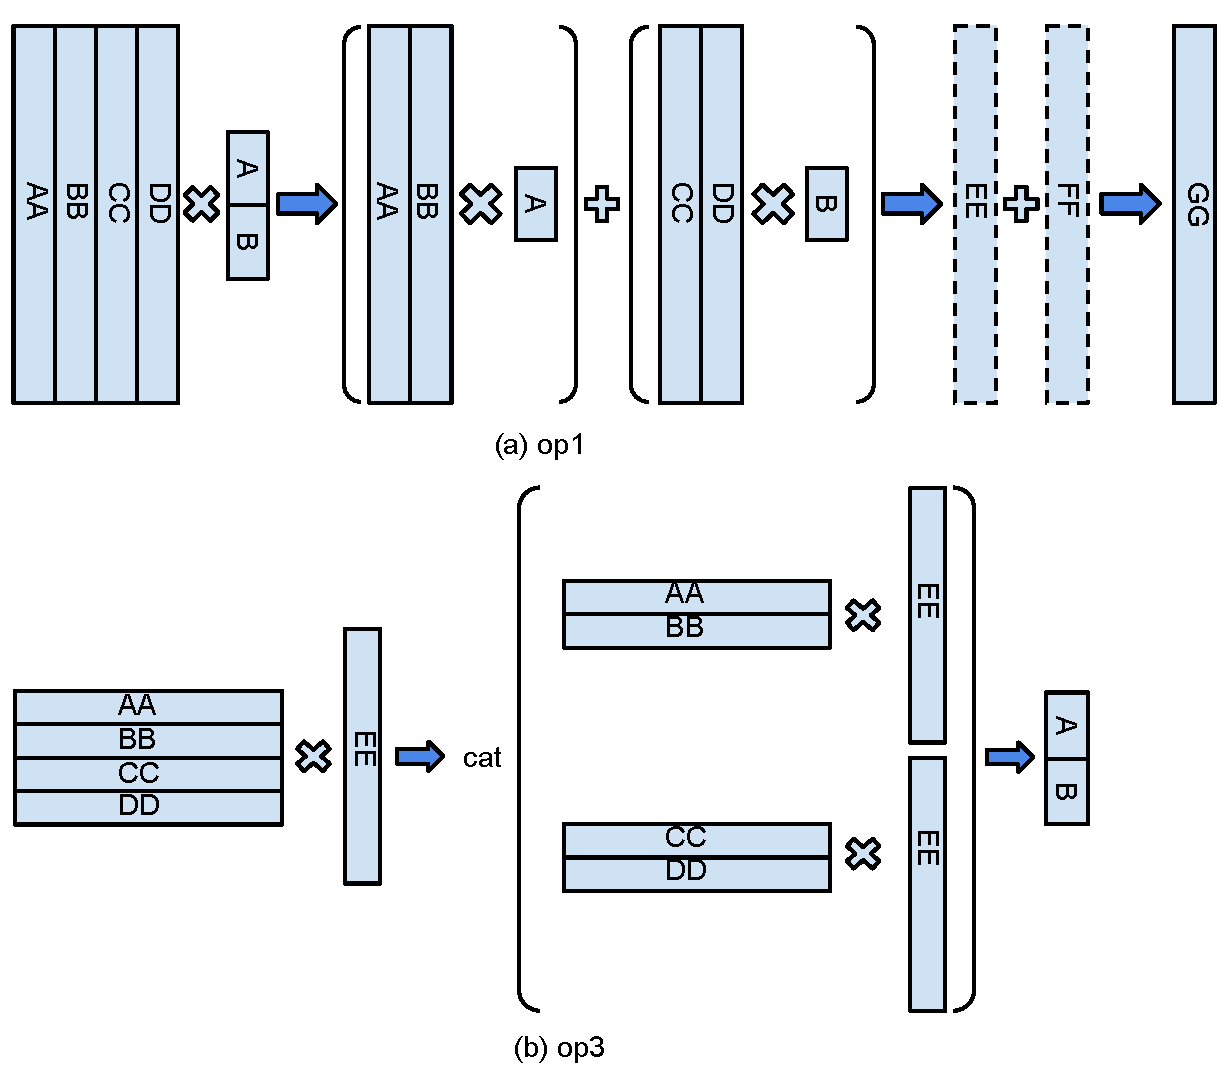
\includegraphics[scale=0.4]{./mat_group.pdf}
\vspace{-5pt}
\caption{Break a large group of dense matrices in an operation into multiple
small groups to reduce memory consumption. XX indicates a TAS matrix
stored on SSDs and X indicates a small matrix stored in memory.}
\vspace{-5pt}
\label{fig:mat_group}
\end{figure}

%\subsubsection{Lazy evaluation} \label{sec:lazy_eval}
%Lazy evaluation avoids materializing every dense matrix to reduce the amount
%of data read and written to SSDs.
%To enable lazy evaluation, we define a special matrix to represent the output
%of a matrix operation. Such a matrix does not store the data of
%an operation result. Instead, it stores the computation and a reference to
%the input matrices. We refer to these special matrices as \textit{virtual matrices}.
%We can evaluate most matrix operations in Table \ref{anasazi_ops} lazily,
%as long as the output matrix of an operation is a TAS matrix. Only \textit{op3}
%and \textit{op6} cannot be evaluated lazily because they output small matrices
%and small vectors stored in Anasazi's native matrices and vectors.

%With \textit{virtual matrices}, we construct a directed acyclic graph (DAG)
%at runtime to represent computation in FlashEigen. In the DAG, we store
%all scalar variables and small matrices as part of computation.
%Figure \ref{comp_seq} shows an example of a sequence of dense matrix operations
%performed in FlashEigen. Figure
%\ref{dag} visualizes the sequence of computation, which forms a directed acyclic
%graph (DAG). Inside this DAG, we do not need to perform any computation other
%than the last one.

%All matrices in FlashEigen are immutable so that \textit{virtual matrices}
%can generate the same result every time when they are materialized. Therefore,
%our implementation of the matrix operations in Table \ref{anasazi_ops} always
%generates new matrices. The original Anasazi matrix operations require in-place
%update on the existing dense matrices, so FlashEigen only passes a pointer to
%a dense matrix to the Anasazi eigensolvers instead of the matrix data.
%This approach is equivalent to variable renaming used by compilers.
%A dense matrix is garbage collected only when there are not any references to
%the matrix.

%\textit{op7} and \textit{op8} access individual columns and have to be incorporated
%with the lazy evaluation. The eigensolvers usually access only one column at a time
%from a dense matrix. When accessing a single column, we materialize the virtual
%matrix in column major if the underlying matrix is a \textit{virtual matrix}.
%Because all matrices are immutable, setting a column in a matrix needs to
%copy the original matrix and set the particular column. Instead of physically
%generating the matrix, we create a virtual matrix that merge the original matrix
%with the column.

%\begin{figure}
%\begin{minted}[mathescape,
%		fontsize=\scriptsize,
%		frame=single,
%]{r}
%# MV0, MV1, MV2, MV3, MV4 are tall dense matrices.
%# B1, B2, B3, B4 are small dense matrices.
%# MV1 is the result of sparse matrix dense matrix
%# multiplication.
%MV0 <- rand_init
%MV1 <- SpMM
%MV2 <- 1 * MV0 * B1 + 0 * MV2
%MV2 <- 1 * MV2 * B2 + 0 * MV2
%MV3 <- 1 * MV1 * B3 + 0 * MV1
%MV1 <- -1 * MV2 * B4 + MV3
%MV4 <- MV1 * diag(vec)
%B <- t(MV4) * MV4
%\end{minted}
%\vspace{-5pt}
%\caption{A small sequence of dense matrix operations typically performed by
%the Anasazi eigensolvers.}
%\label{comp_seq}
%\end{figure}

%\begin{figure}
%\centering
%\includegraphics[scale=0.5]{./dag.pdf}
%\vspace{-5pt}
%\caption{A directed acyclic graph represents the sequence of matrix operations
%shown in Figure \ref{comp_seq}. Each rounded rectangular node indicates
%a virtual matrix and each rectangular node indicates a materialized matrix.}
%\vspace{-5pt}
%\label{dag}
%\end{figure}

%To perform actual computation, FlashEigen needs to materialize
%\textit{virtual matrices}. It materializes a \textit{virtual matrix} when
%encountering \textit{op3} and \textit{op6} because these two operations
%output Anasazi's native matrices and vectors.
%A \textit{virtual matrix} represents some computation on some materialized
%TAS matrices stored on SSDs. FlashEigen materializes
%a \textit{virtual matrix}, which has more than one materialized input matrix,
%to minimize the amount of data read from SSDs.
%FlashEigen also materializes all of the dense matrices in the basis.

%A \textit{virtual matrix} may contain a sequence of operations, so materializing
%it may trigger matrix materialization recursively. We discard the materialized
%partition of an intermediate matrix, once it is no longer needed, to avoid
%writing data of an intermediate matrix to SSDs.
%We partition a \textit{virtual matrix} horizontally in the same fashion as
%the external-memory matrices and materialize each partation independantly. 
%To increase CPU cache hits, we use a much smaller partition size than
%the external-memory matrix. As such, the output of the previous operation is
%still in the CPU cache when it is fed to the next operation.

\subsubsection{Matrix caching}
FlashEigen deploys two forms of matrix caching to reduce I/O to SSDs.
In the first case, FlashEigen worker threads cache part of a TAS
matrix locally. In the other case, FlashEigen can also cache the most recent
TAS matrix in the vector subspace.

Caching part of a TAS matrix read from SSDs benefits some of
the matrix operations. One example is the optimization for $op3$ in section
\ref{sec:em}, which breaks a large group of dense matrices into multiple
subgroups and the matrix in the right operand is shared by all of the subgroups.
A worker thread only needs to cache data in a row interval of the right matrix
that is currently being processed because a thread processes one row interval
at a time and each row interval of the TAS matrices is processed only once.
Therefore, a worker thread can buffers the data in a row interval of a matrix
locally and accessing the buffered data doesn't incur any locking overhead.

When we buffer the recent portions, we need to give each matrix a data identifier
to identify its data, so we can recognize which portion of data can be reused.
For certain operations, even though a new matrix is created, the data inside
remains the same. A typical example is transpose. The identifier we give to
each matrix should identify the data inside a matrix instead of individual matrices,
so a transposed matrix and its original matrix should share the same identifier.

FlashEigen also caches the most recent TAS matrix in the vector subspace if
the RAM of a machine is sufficient to accommodate the entire matrix.
When a new matrix in the vector subspace is generated by sparse matrix
multiplication, an eigensolver needs to perform a sequence of operations on it,
which includes reorgonalization. By caching the matrix in memory, we can
significantly reduce the amount of data written to SSDs.

\subsection{Discuss memory and I/O complexity.}
The lower bound of memory consumption is O(n). i.e., we keep a single vector
in memory.
